\documentclass[preprint,authoryear,12pt]{elsarticle}

\usepackage{amsmath}
\usepackage{aas_macros}
\usepackage{rotating}
\usepackage{xspace}
\usepackage{booktabs}
\usepackage{multirow}
\usepackage{color}
\usepackage{listings}
\usepackage{caption}
\usepackage{url}
\journal{Astronomy and Computing}

%%% Definitions added by Manodeep 
\newcommand{\Msun}{M_{\odot}}
\newcommand{\hMsun}{h^{-1}M_{\odot}}
\newcommand{\sdss}{{\small{SDSS}}\xspace}
\newcommand{\hMpc}{\ensuremath{{h^{-1}Mpc}\xspace}}
\newcommand{\hkpc}{\ensuremath{{h^{-1}kpc}\xspace}}
\newcommand{\emcee}{\texttt emcee}
\newcommand{\rmax}{\ensuremath{{r_{max}}}\xspace}
\newcommand{\xir}{\ensuremath{{\xi(r)}}\xspace}
\newcommand{\wprp}{\ensuremath{{w_p(r_p)}}\xspace}
\newcommand{\xirppi}{\ensuremath{{\xi(r_p,\pi)}}\xspace}
\newcommand{\todo}[1]{\marginpar{TODO}{\color{red}#1}}



\lstset{
  language=C,                % choose the language of the code
  basicstyle=\ttfamily,      % sets font
  numbers=left,                   % where to put the line-numbers
  numberstyle=\small, 
  stepnumber=1,                   % the step between two line-numbers.
  numbersep=10pt,                  % how far the line-numbers are from the code
  backgroundcolor=\color{white},  % choose the background color. You must add \usepackage{color}
  showspaces=false,               % show spaces adding particular underscores
  showstringspaces=false,         % underline spaces within strings
  showtabs=false,                 % show tabs within strings adding particular underscores
  tabsize=2,                      % sets default tabsize to 2 spaces
  captionpos=b,                   % sets the caption-position to bottom
  breaklines=true,                % sets automatic line breaking
  breakatwhitespace=true,         % sets if automatic breaks should only happen at whitespace
}

\begin{document}

\begin{frontmatter}

\title{Cache is King: Presenting a Suite of Fast, Correlation Function Codes}

\author[ms]{Manodeep Sinha}
\ead{manodeep.sinha@vanderbilt.edu}
\address[ms]{6902 Stevenson Center, Department of Physics \& Astronomy, Vanderbilt University, Nashville, TN 37235}

\begin{abstract}
We have entered the era of `Big Data' where we are gathering a tremendous amount of data that
needs to be processed as well as modeled accurately. In particular, large galaxy surveys
like the Sloan Digitial Sky Survey requires computing correlation functions. While measuring the
correlation function in the data is not a bottle-neck, modeling the observed galaxy distribution correctly
{\em} requires a MCMC chain and repeated measurements of $\xi(r)$ and/or $\xi(r_p,\pi)$. However, 
the architecture of modern CPU's means that best performance is only obtained when cache misses 
are kept to a minimum. Here, I present a suite of 3 correlation function codes that exploit 
current CPU architecture and hand-written AVX  


The accompanying codes are publicly available at \url{https://bitbucket.org/manodeep/Corrfunc/}. 
\end{abstract}

\begin{keyword}
methods: numerical \sep (cosmology:) large-scale structure of universe \sep
\end{keyword}

\end{frontmatter}

\section{INTRODUCTION}
%% %% MS: I have not encountered this in the past -- but the footnotecounter needs to be reset. Otherwise, 
%% %% the numbering starts at Nauthors+1. Presumably \altaffiltext uses \footnote internally and does not
%% %% reset the counter like a responsible person!
%% \setcounter{footnote}{0}
The large-scale structure of the Universe can be now measured using $\mathcal{O}$(million) galaxies 
using data from current surveys like SDSS/BOSS surveys. Upcoming surveys like LSST will probe even 
deeper and wider and aim to target on $\mathcal{O}$(10's of million) galaxies. With such a large galaxy data, 
we can measure the galaxy density field fairly accurately in the data. While the number of galaxies observed 
in these current and upcoming surveys is large, we have to compute the galaxy density fields {\em only once}. Thus, 
even a slow, correlation function code will be fine when measuring the data correlation function. 
However, predicting this galaxy  density field data will require an even larger number of model galaxies -- increasing the computational 
load of determining the density field even further. Typically, the modeling process also involves an MCMC -- 
requiring $\sim$ millions of evaluations of the correlation function.\footnote{I will assume that creating the models themselves 
is much faster compared to computing the correlation functions.} 

Modern cpu's have a hierarchy of memory locations; the smallest and fastest are closest to the cores while the largest and slowest are the
farthest. All cpu instructions need to be carried out from cpu registers - there are $\sim 10-30$ registers typically available and the 
access times can be thought of as instantaneous. Next up is the $L1$ cache divided into $L1D$ for data and $L1I$ for instructions cache. Since 
the cpu always necessarily executes instructions that are close together, we will ignore the instruction cache from now on. Typical $L1$ cache 
sizes range from 64KB to 128 KB. Next level up is the $L2$ cache, typically $\sim$ 256KB to 1 MB. The last level cache or the $L3$ cache 
is usually shared across all cores on the socket and can be 10 MB to 40 MB. 


\section{Methods}
We need to compute pairwise distances to get the correlation function. A naive implementation of a correlation function would compute {\em all possible} 
pairwise separations with a complexity $\mathcal{O}(N^2)$. However, for almost all correlation functions, we are only interested in separations less than 
a certain \rmax, where \rmax is much smaller than the domain of the point distribution itself. We can then immediately see a way to prune pairs that can not
{\em possibly} be within \rmax. If we impose a 3-d grid, with cell-size \rmax, then two points separated by more than one cell size (\rmax) in any one 
dimension can not be within \rmax of each other. Thus, given one point which is the target galaxy and a grid with cell-size \rmax, 
immediately allows us to prune {\em all} of the points that are not within 1 cell offset in each dimension. However, even with this pruning, the actual 
implementation of the algorithm matters. For instance, a linked-list in each cell performs $\sim 60\times$ worse than the algorithm described here.\footnote{The 
usual linked-list is very cache-unfriendly. Each dereference requires a read from a new region of memory and an almost guaranteed cache miss. } 

\subsection{Partitioning the Particles based on \rmax}

\begin{figure}[htbp]
\centering
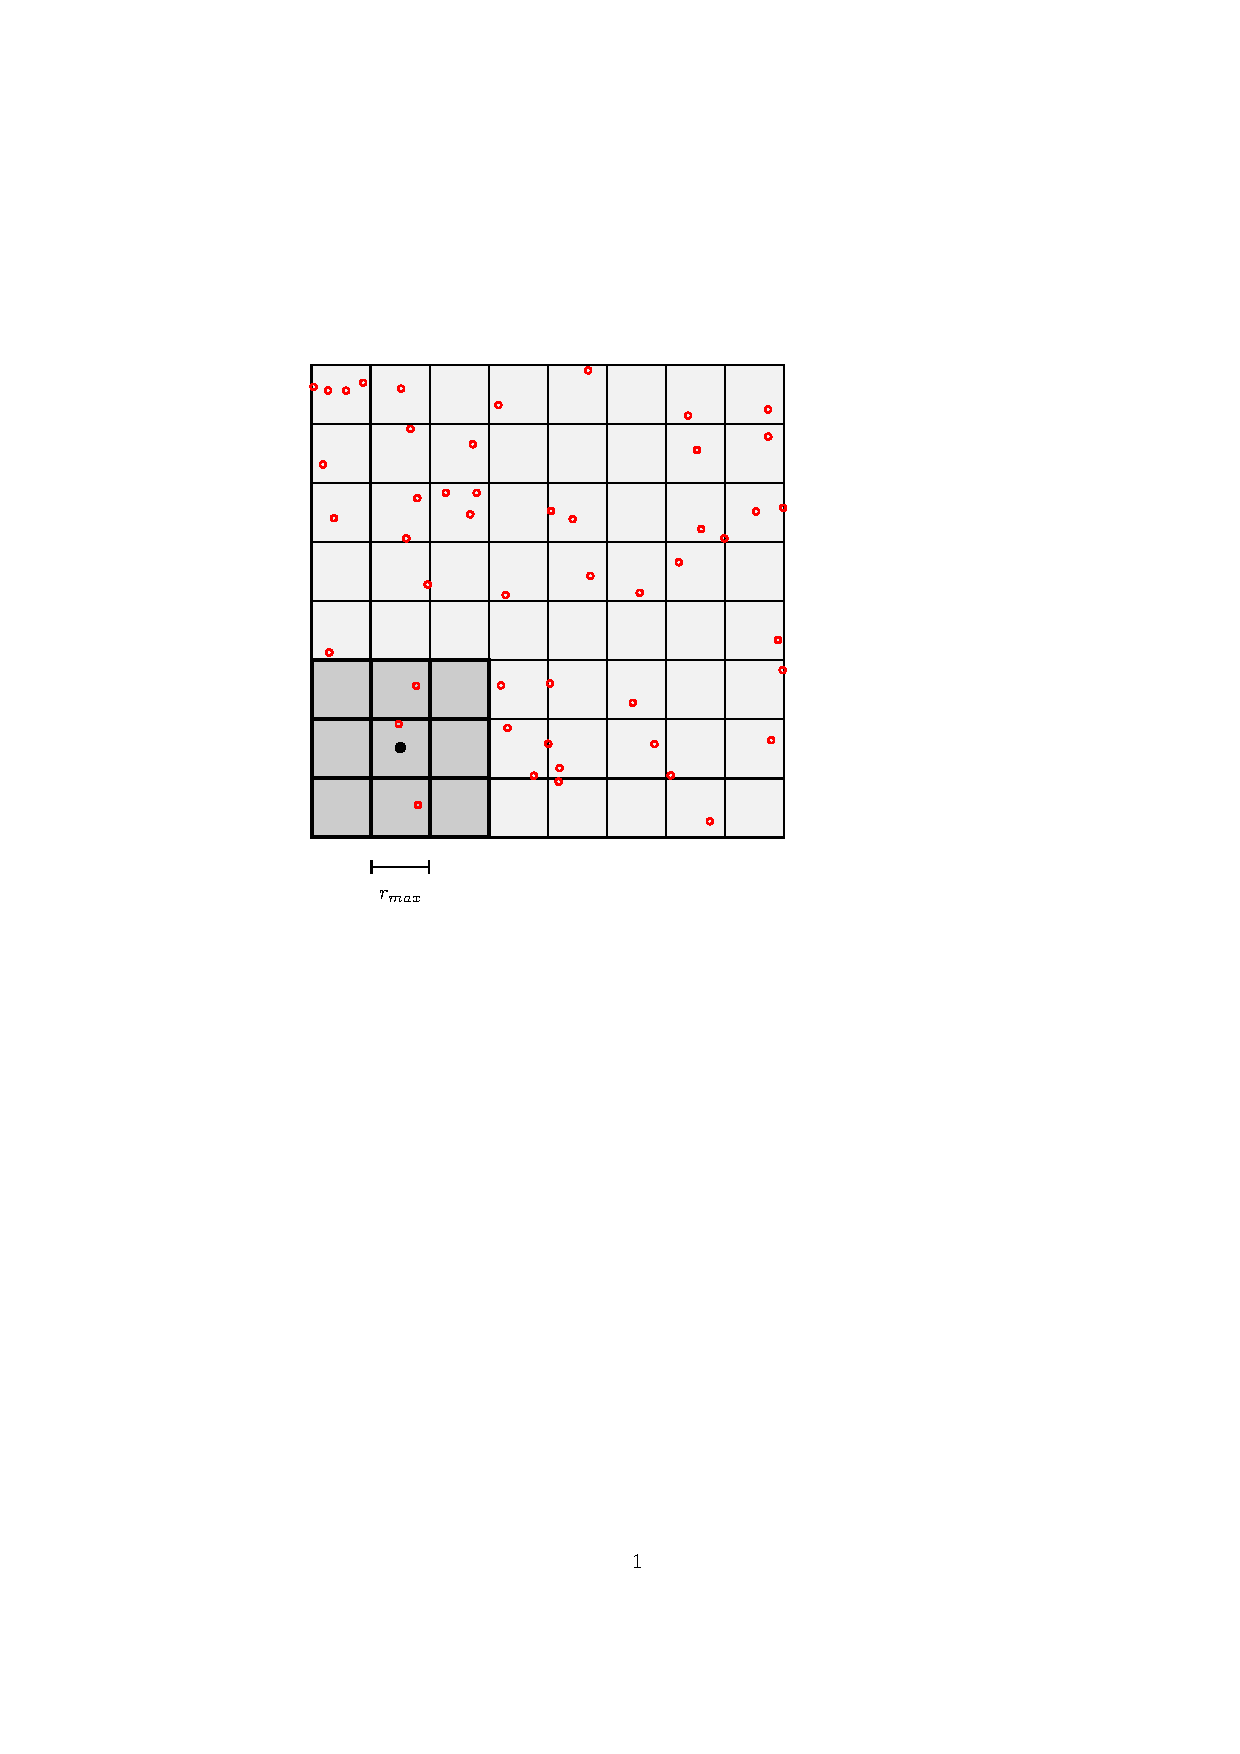
\includegraphics[clip=true]{tikz_grid}
\caption{A 2-D grid showing the bin-lattice partitioning scheme. The bigger square show the entire 
domain, the red circles show a random distribution of 100 particles. Let's say we want to compute all pairs 
for the target blue point, then we would only have to consider red points that are within one cell (the dark shaded region). 
A circle with radius \rmax is also drawn to shown the actual pairs that will eventually count in the correlation function.} 
\end{figure}


\subsection{How to Maintain Cache Locality within the Grid}
For all pairs around a given target galaxy, we need to compute distances to all points within all neighbouring 3-d cells. 
We ensure that the particle locations are contiguous by moving them into the following \texttt{C struct} in the order in which they arrive. 

\begin{lstlisting}
typedef struct{
  DOUBLE *x;
  DOUBLE *y;
  DOUBLE *z;
  int64_t nelements;
} cellarray;
\end{lstlisting}

Since the typical particle data is small ($\sim$ 20-30 MB), duplicating the entire particle distribution does not impose a strong 
constraint on the memory requirements. However, this duplication allows us to store the particles contiguously and produces fewer 
cache misses while looping over particles in a cell. 
The entire 3-D particle distribution is then deposited on the uniform grid. Now, for each particle we need to visit 27 total cells to 
compute all possible pairs within \rmax. 

\section{The pair-counting algorithm}

\subsection{\xir}
\subsection{\xirppi}
\subsection{\wprp}

\subsection{Hand-written Vectorization Support}
Advanced Vector Extensions (AVX) has been available in cpu's more recent than 2011. AVX allows the processing of 8 floats or 4 double simultaneously -- thus, 
potentially increasing the throughput by a factor of 8x/4x. However, automatic vectorization is not always possible by the compiler and in those cases 
we can write AVX vector intrinsics to directly manipulate 8 floats/4 doubles\footnote{Another option would be to use the vectorclass written by Agner Fog here: \url{http://agner.org/optimize/vectorclass/}}. 


\section{Benchmarks \& Scaling}
In this section we present the runtimes and scalings for different number of particles, \rmax and OpenMP threads for the codes. 
For all of the scaling tests, only an auto-correlation calculation was used and the fiducial catalog contains $\sim 1.2$ million 
galaxies on a periodic cube of side 420 \hMpc. 

\subsection{Scaling with Number of Particles}
In Fig.~\ref{fig:scaling_numpart}, we show the scaling for the three codes with the number of particles. For this scaling, we subsampled 
the fiducial mock to attain 10 logarithmic steps in particle number ranging from $1.2\times10^4$ to $1.2\times10^6$. 

\begin{figure}[htbp]
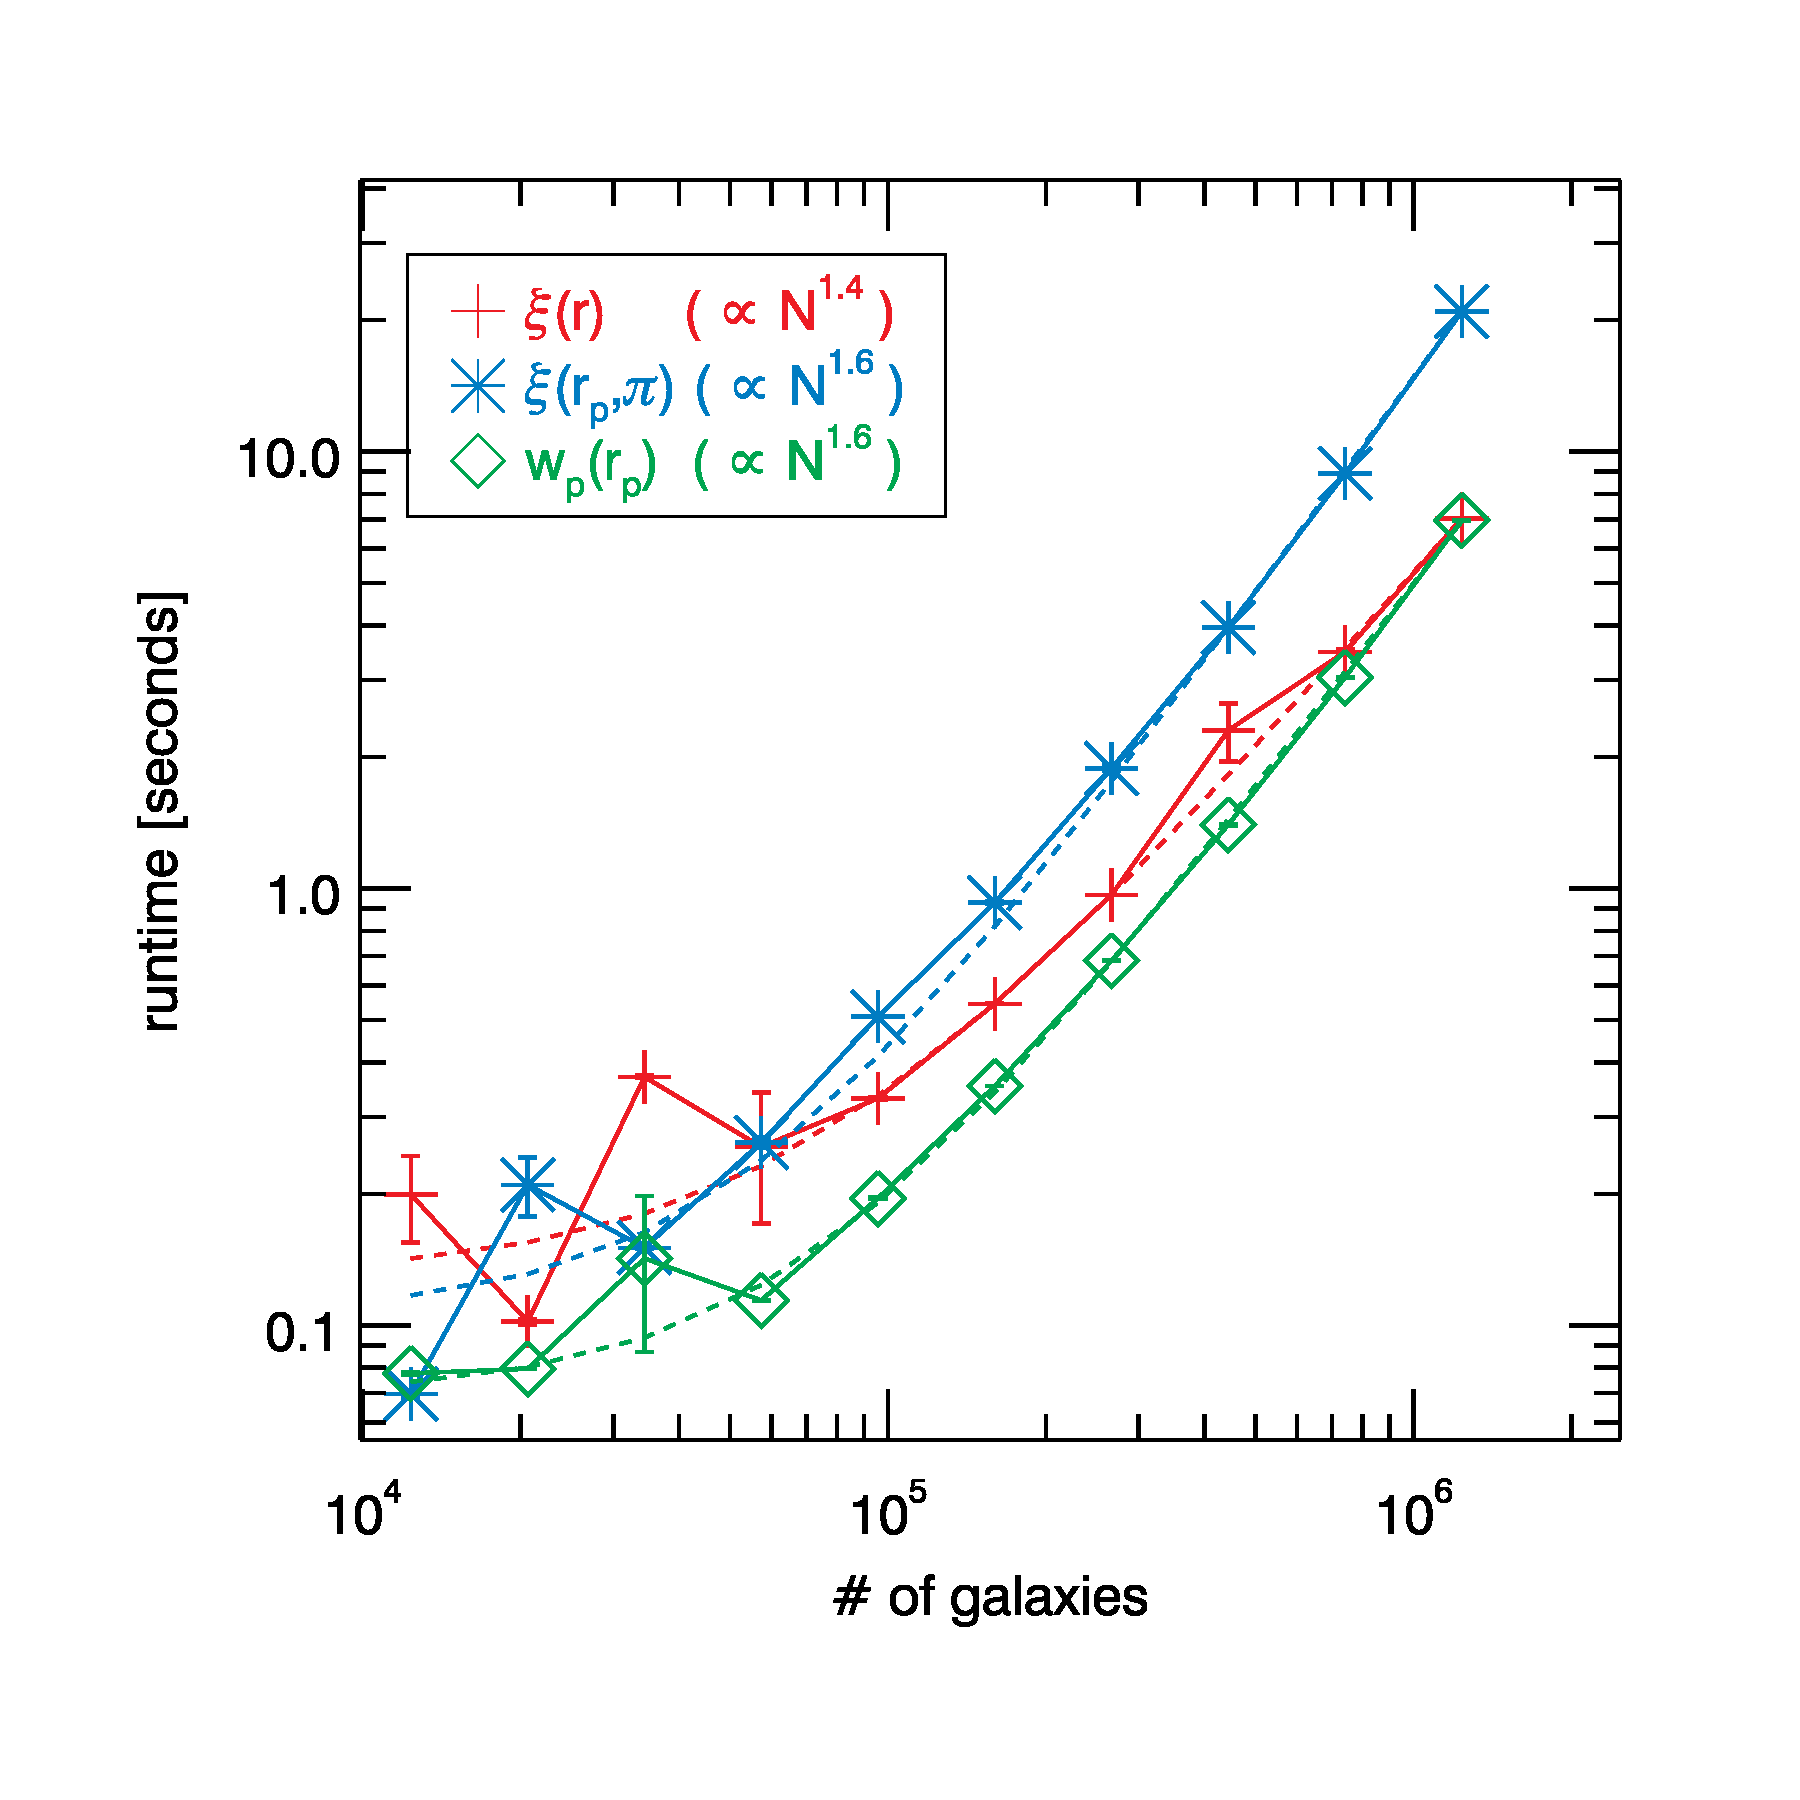
\includegraphics[clip=true,width=\linewidth]{timings_Mr19_numpart}%
\caption{Scaling with particle number for \xir, \xirppi, \wprp }
\label{fig:scaling_numpart}
\end{figure}

\subsection{Scaling with \rmax}
\begin{figure}[htbp]
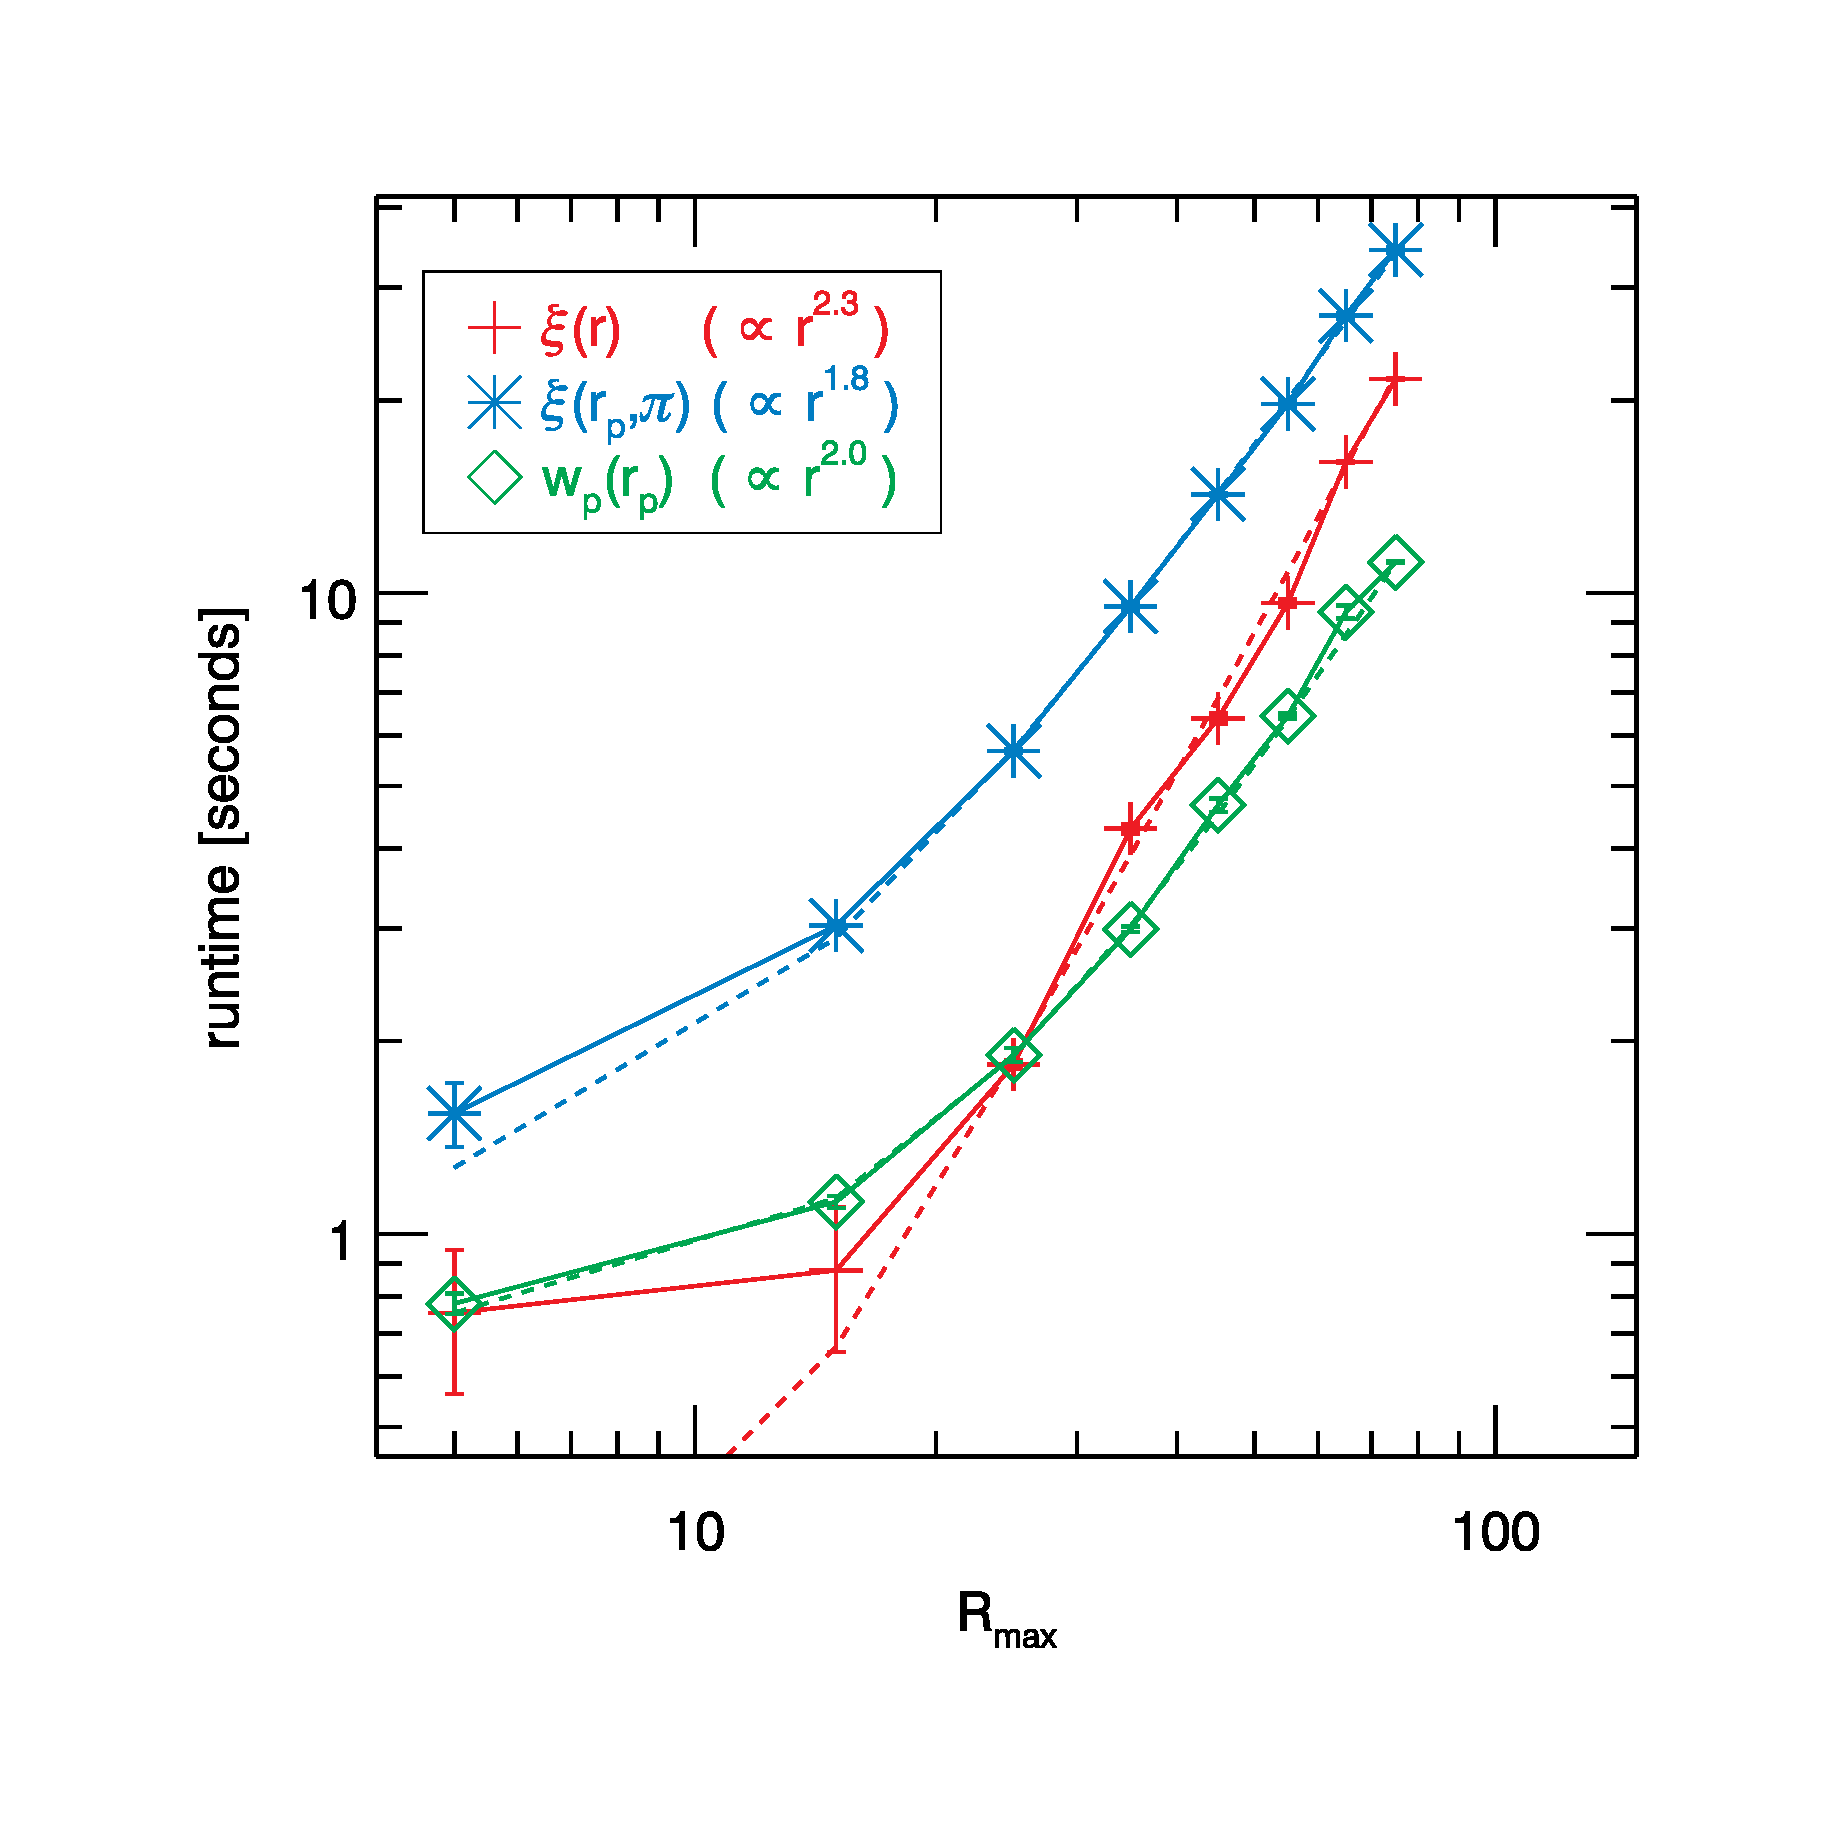
\includegraphics[clip=true,width=\linewidth]{timings_Mr19_rmax}%
\caption{Scaling with \rmax for \xir, \xirppi, \wprp }
\label{fig:scaling_rmax}
\end{figure}


\subsection{Scaling with OpenMP threads}
\begin{figure}[htbp]
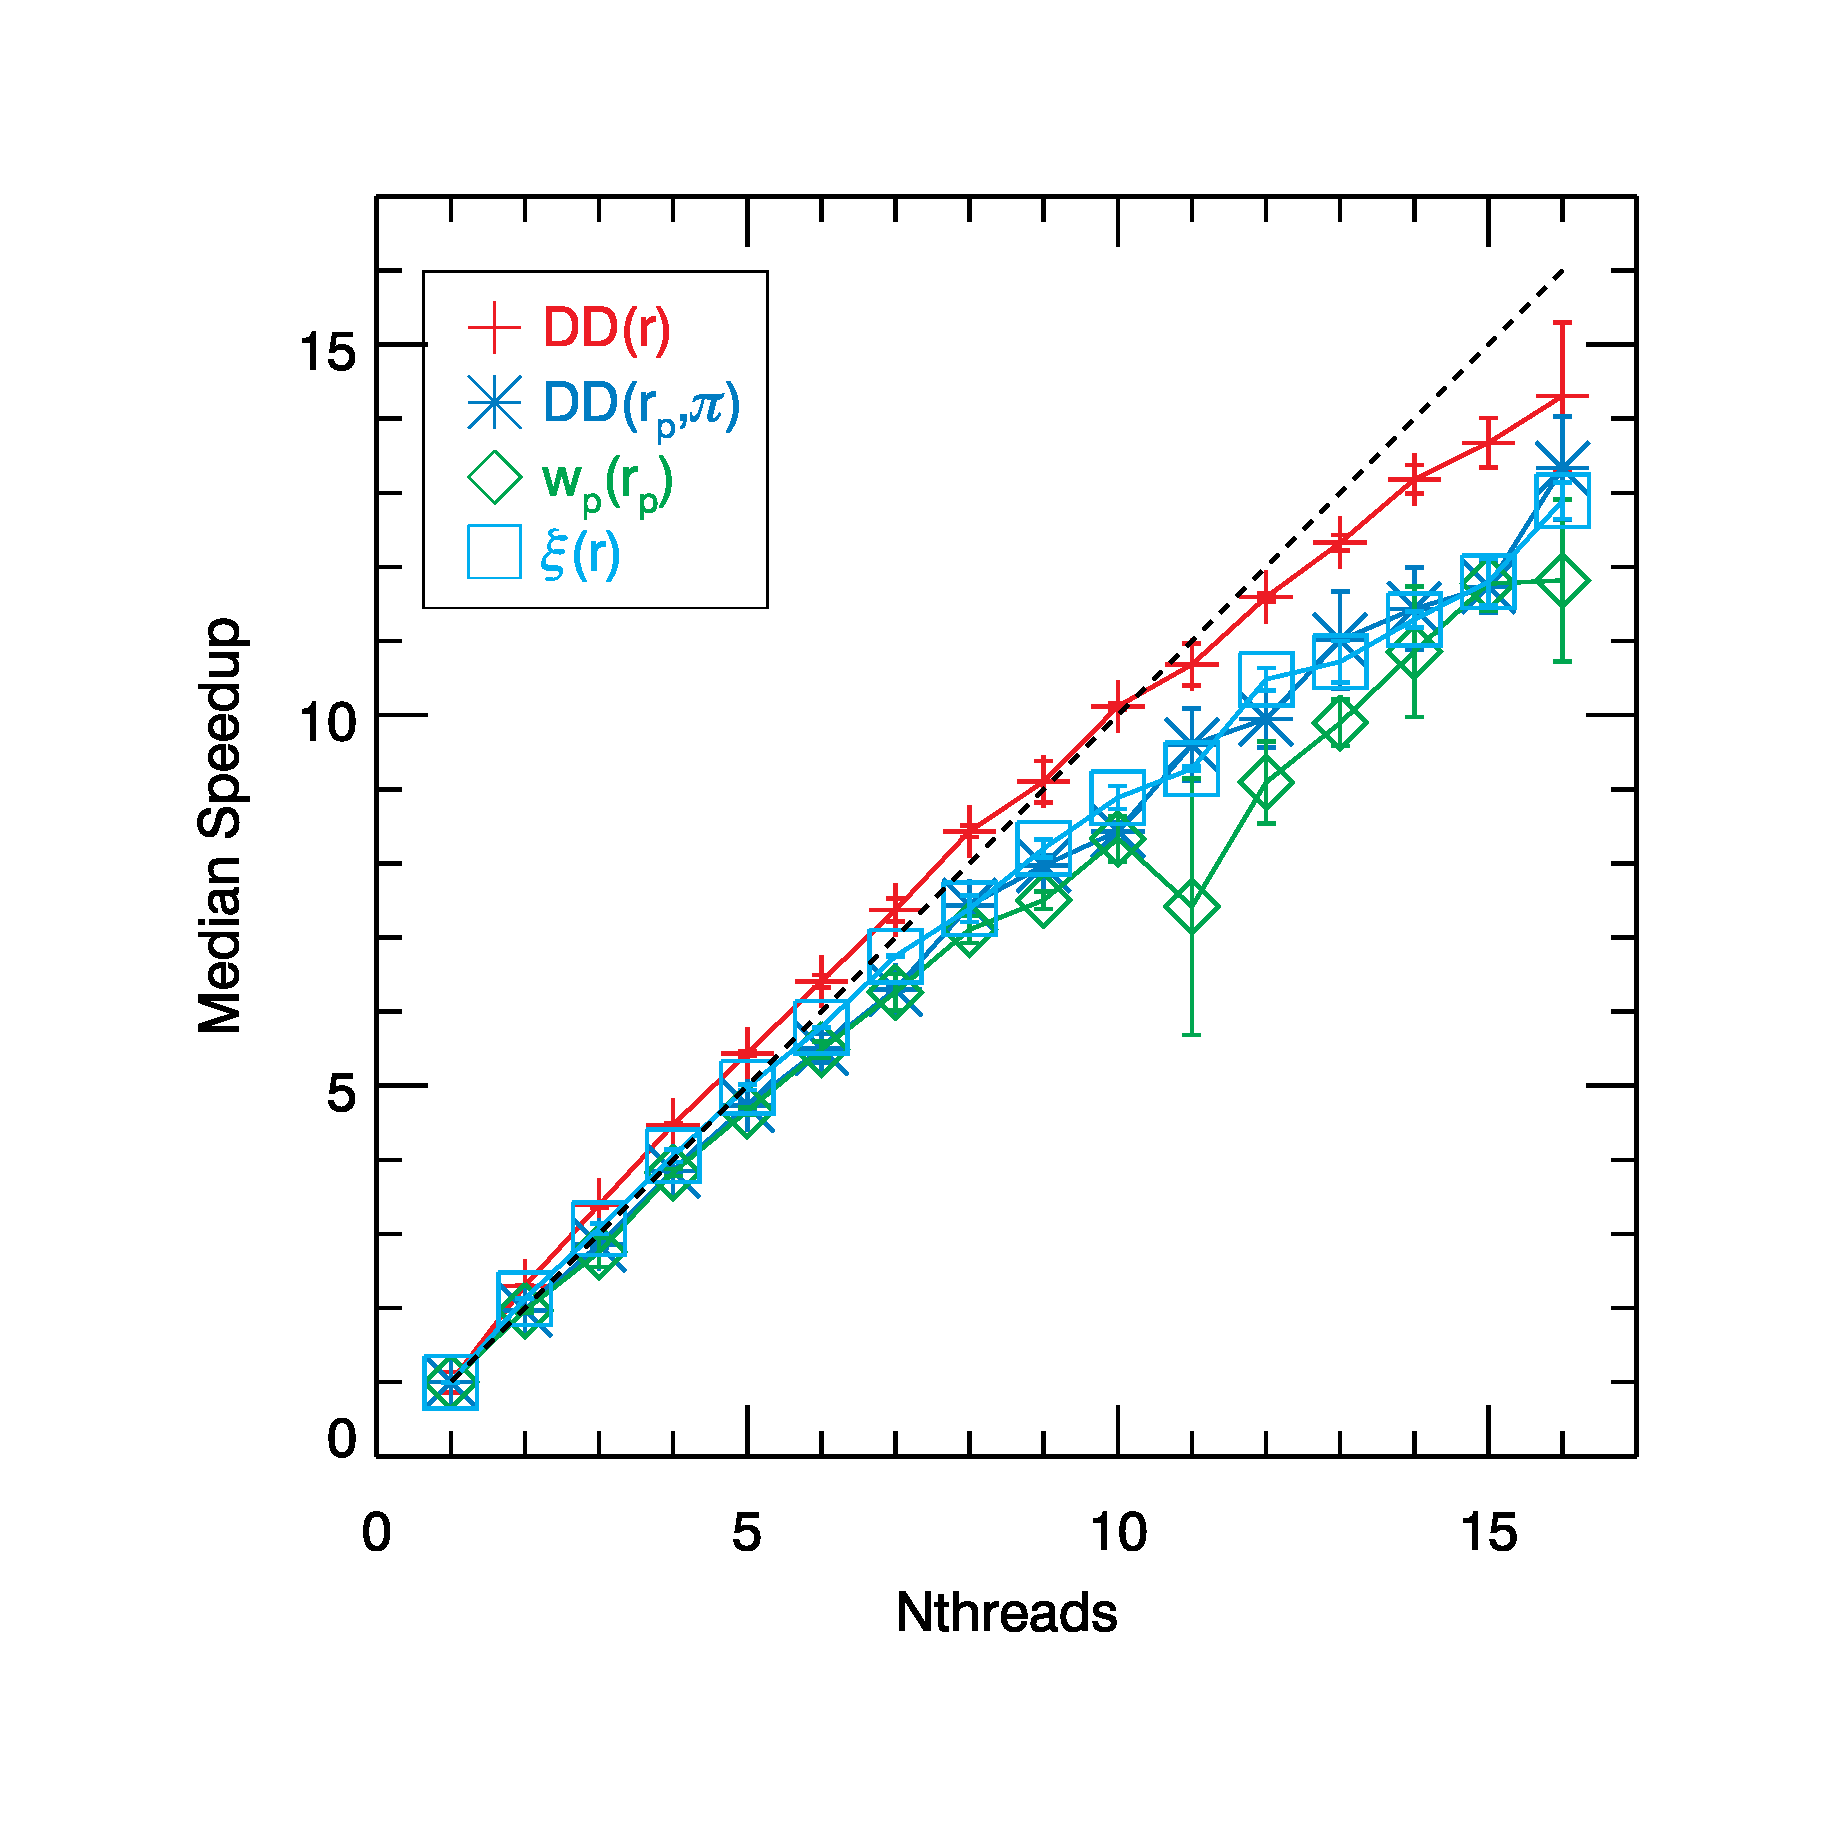
\includegraphics[clip=true,width=\linewidth]{timings_Mr19_openmp}%
\caption{OpenMP scaling for \xir, \xirppi, \wprp }
\label{fig:scaling_openmp}
\end{figure}

\section{Conclusions}
I have presented a suite of three fast correlation function codes that take advantage of the underlying hardware. The reasons why the codes 
are much faster for typical workloads are:
\begin{itemize}
\item A `bin-lattice' scheme is used to first partition the computational domain into 3-D cells that can then be used to prune majority of the volume. 
\item To obtain better cache-locality, the particle list is duplicated into a contiguous array for each dimension. Thus, all particles that fall into the
same 3-D cell are stored in a contiguous array. 
\item With the AVX instruction set, modern CPU's can process 8 floats/4 doubles simultaneously. The codes contain hand-written AVX intrinsics that offer a 
factor of few speedup compared to the compiler generated scalar code. 
\end{itemize}

\citet{foreman-mackey_etal_13}

\section*{Acknowledgements}

\bibliographystyle{elsarticle-harv}
\bibliography{master}

\end{document}




